\chapter{\label{ch:methodology} Methodology}
This chapter outlines the methodology employed throughout the lifecycle of this project, focusing on the system architecture, design choices, and integration of key subsystems in achieving the overall project objectives. Each design decision is supported by a brief mention of relevant literature and appropriate system requirements, further analysis on component/algorithm selection can be found in Chapter \ref{ch:ch4}.

\section{\label{sec:overview} Overview}

The mobile robot project is structured around several interconnected subsystems, which work together to achieve real-time autonomous navigation, user interaction through AR markers, and remote control via a web interface. A high-level diagram (Figure \ref{fig:high_level_diagram}) visualizes this architecture, comprising a Raspberry Pi (as the main processor), a camera module, motor control, AR-based fiducial marker detection, and a web-based user interface. 

\begin{figure}[h]
	\centering
	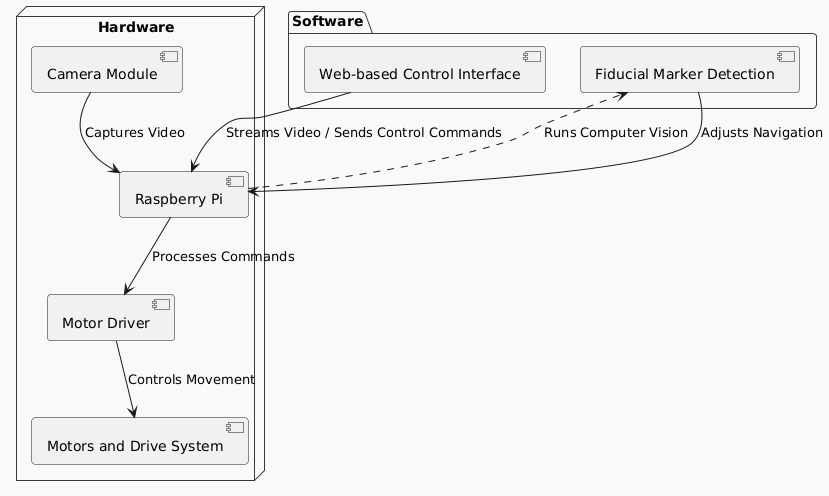
\includegraphics[width=0.9\textwidth]{ch3/figs/diagram.png}
	\caption{High Level Diagram of Project Architecture}
	\label{fig:high_level_diagram}
\end{figure}


The system begins with the camera capturing video streams, processed by the Raspberry Pi for AR marker recognition and navigation. Simultaneously, the web interface allows remote commands to be issued and video feedback to be streamed, closing the control loop between the user and the robot. This methodology draws inspiration from similar studies, such as La Delfa et al. \cite{delfa2015} and Jacobsen et al. \cite{jacobsen2018}, which explore mobile robots with AR capabilities.

As outlined in Section \ref{sec:objectives}, the system needs to meet specific requirements to ensure it performs as intended. These requirements were established through research, discussions with supervisor, and analysis of the intended user environment.

\begin{table}[h]
	\centering
	\begin{tabular}{|p{0.9cm}|p{6cm}|p{0.9cm}|p{6cm}|}
		\hline
		\textbf{Req. ID} & \textbf{Requirement Description}                                                                                                                                    & \textbf{Spec. ID} & \textbf{Specification Description}                                                                                                        \\ \hline
		\textbf{R1}      & The robot must operate in different control zones, defined by AR markers, and adjust its behavior accordingly (e.g., slowing down, stopping, or performing a task). & \textbf{F1}       & Implementation of AR-based control zones that dynamically adjust robot speed, direction, or initiate tasks based on detected markers.     \\ \hline
		\textbf{R2}      & The system must integrate dynamic instructions based on ArUco marker detection, allowing for real-time task updates.                                                & \textbf{F2}       & Real-time processing of ArUco markers to update task instructions and provide context-specific navigation and task execution.             \\ \hline
		\textbf{R3}      & The AR interface must provide real-time visual feedback for the human operator to improve task monitoring and control.                                              & \textbf{F3}       & AR-based visual feedback will provide the human operator with real-time monitoring of the robot’s actions and environmental interactions. \\ \hline
		\textbf{R4}      & The robot must include object avoidance functionality, ensuring it maintains a safe distance from recognized obstacles (e.g., warning cones) based on AR markers.   & \textbf{F4}       & Integration of object avoidance behavior, ensuring the robot maintains a safe distance from obstacles based on AR marker detection.       \\ \hline
		\textbf{R5}      & The system should detect and respond to wheel slip events caused by changes in surface traction, providing stability during operation.                              & \textbf{F5}       & Implementation of wheel slip detection functionality that monitors the robot's power draw to identify surface traction changes.           \\ \hline
	\end{tabular}
	\caption{Requirements and Functionalities for the Robot Control System}
	\label{tab:requirements_functionalities}
\end{table}


The system begins with the camera capturing video streams, processed by the Raspberry Pi for AR marker recognition and navigation. Simultaneously, the web interface allows remote commands to be issued and video feedback to be streamed, closing the control loop between the user and the robot. This methodology draws inspiration from similar studies, such as La Delfa et al. \cite{delfa2015} and Jacobsen et al. \cite{jacobsen2018}, which explore mobile robots with AR capabilities.

\section{\label{sec:subsystems} Subsystems Overview}
The robot's subsystems are designed to work in tandem, each playing a crucial role in delivering the overall project’s functionality. Below, we discuss the primary subsystems and their respective roles.

\subsection{\label{subsec:camera} Camera Module}
The camera module captures real-time video, which is essential for detecting AR markers and obstacles. Positioned to maximize environmental visibility, the camera's data feeds directly into the Raspberry Pi, where real-time processing occurs. High-definition video capture ensures accurate marker detection and obstacle avoidance, critical for achieving precise navigation.

\textbf{Justification:} The camera module is essential for both marker detection and obstacle avoidance, as demonstrated by Vanitha et al. \cite{vanitha2016}, who emphasize the importance of high-resolution visual input in autonomous systems.

\subsection{\label{subsec:raspberry} Raspberry Pi}
The Raspberry Pi serves as the central processing unit (CPU), handling video input from the camera, running image processing algorithms (via OpenCV), and controlling the motors based on user commands and AR markers. It was selected due to its computational power, affordability, and strong compatibility with the system’s software and hardware requirements. The Pi also facilitates real-time communication between the robot and the web-based interface.

\textbf{Justification:} The Raspberry Pi was chosen over alternatives (e.g., Arduino) for its ability to handle computationally expensive tasks like image processing while maintaining efficient communication with external interfaces, as supported by Jacobsen et al. \cite{jacobsen2018}.

\subsection{\label{subsec:motor} Motor Driver and Drive System}
The motor driver receives commands from the Raspberry Pi and translates them into movements. Pulse-width modulation (PWM) enables precise control of speed and direction, which is essential for executing tasks like AR-based navigation or obstacle avoidance.

\textbf{Justification:} PWM control provides the necessary flexibility for dynamic responses, particularly when navigating through AR-defined zones or avoiding obstacles. Previous work by La Delfa et al. \cite{delfa2015} highlights the significance of precise motor control in mobile robots.

\subsection{\label{subsec:web_interface} Web-Based Control Interface}
The web interface allows for remote control of the robot and streams real-time video to the user. It facilitates direct interaction by allowing users to send movement commands and receive immediate visual feedback. This subsystem is integral for monitoring and controlling the robot's behavior from a distance.

\textbf{Justification:} Real-time feedback and control are critical for AR-based robotics applications, particularly in environments where direct line-of-sight control is impractical. The web-based control interface ensures the system's usability aligns with these requirements, supported by findings from Vanitha et al. \cite{vanitha2016}.

\subsection{\label{subsec:marker_detection} Fiducial Marker Detection}
AR markers, specifically ArUco markers, are used to guide the robot’s navigation. The Raspberry Pi processes the video input using OpenCV, detecting these markers to trigger predefined actions, such as altering the robot’s path or stopping at specified zones.

\textbf{Justification:} Fiducial markers are a reliable, low-cost solution for guiding robotic navigation, as demonstrated by La Delfa et al. \cite{delfa2015}. Their accuracy in marker detection enables real-time adjustments, which are crucial for dynamic interaction with the environment.

\subsection{\label{subsec} Obstacle Detection} 
Obstacle detection is critical for ensuring the safe navigation of the robot in dynamic environments. This process leverages computer vision techniques, specifically using a YOLO (You Only Look Once) model, to identify and localize obstacles such as bottles or other potential hazards in real-time. The Raspberry Pi captures video input from a camera mounted on the robot, and the YOLO model processes each frame to detect obstacles.

\textbf{Justification:} Implementing YOLO for obstacle detection allows for efficient processing of video frames and quick responses to dynamic environments. According to Redmon et al. \cite{redmon2015}, YOLO achieves state-of-the-art performance in object detection by balancing speed and accuracy, making it suitable for real-time applications in robotic systems. This capability enables the robot to navigate autonomously while avoiding collisions, enhancing overall operational safety and efficiency.


\section{\label{sec:interaction} Interaction and Dependencies}
The subsystems work in unison to create a seamless experience for both the robot and the user. The camera module captures the environment, with the Raspberry Pi processing the video stream to detect fiducial markers. The Pi sends commands to the motor driver to adjust the robot’s movement while relaying the processed video to the web-based control interface, allowing for user feedback and control. This integration is essential to ensure that navigation, interaction, and feedback are synchronized and responsive to both user input and environmental changes.

\section{\label{sec:atp} Acceptable Test Procedures (ATP)}
The success of the project depends on thorough testing of each subsystem. The tests are designed to ensure the system meets its functional and performance requirements. Table \ref{tab:testing} outlines key test scenarios linked to specific subsystems and project goals, ensuring the robot performs as expected in various operational conditions.

\begin{table}[ht]
	\centering
	\caption{Enhanced Breakdown of sub-tests to be performed in the acceptance testing.}
	\label{tab:testing}
	\begin{tabular}{|p{0.8cm}|p{3.6cm}|p{7.5cm}|p{0.9cm}|p{0.9cm}|}
		\hline
		\textbf{Test} & \textbf{Description}                                           & \textbf{Expected Outcome}                                                                                                                          & \textbf{Spec. ID} & \textbf{Req. ID} \\ \hline
		T1            & Test the robot’s behavior in AR-based control zones            & The robot adjusts speed or direction based on AR markers within defined zones (e.g., slow zone, stop zone).                                        & F1                & R1               \\ \hline
		T2            & Test real-time ArUco marker detection for dynamic instructions & Robot recognizes ArUco markers in real-time and triggers corresponding task instructions (e.g., task initiation or environmental change response). & F2                & R2               \\ \hline
		T3            & Test AR-based visual feedback for real-time monitoring         & The user receives accurate and real-time AR feedback on the robot’s position, detected markers, and current task.                                  & F3                & R3               \\ \hline
		T4            & Test object avoidance system using visual markers              & The robot successfully avoids predefined obstacles marked by ArUco codes within 20 cm, halting or rerouting its path.                              & F4                & R4               \\ \hline
		T5            & Test wheel slip detection and response functionality           & The robot detects slip on different surfaces (e.g., sand or wet surfaces) and compensates by adjusting motor power or stopping.                    & F5                & R5               \\ \hline
	\end{tabular}
\end{table}

